% Insert the first figure in Corpus construction, immediately after
% Table~\ref{tab:final-corpus}.

\begin{figure}[H]
    \centering
    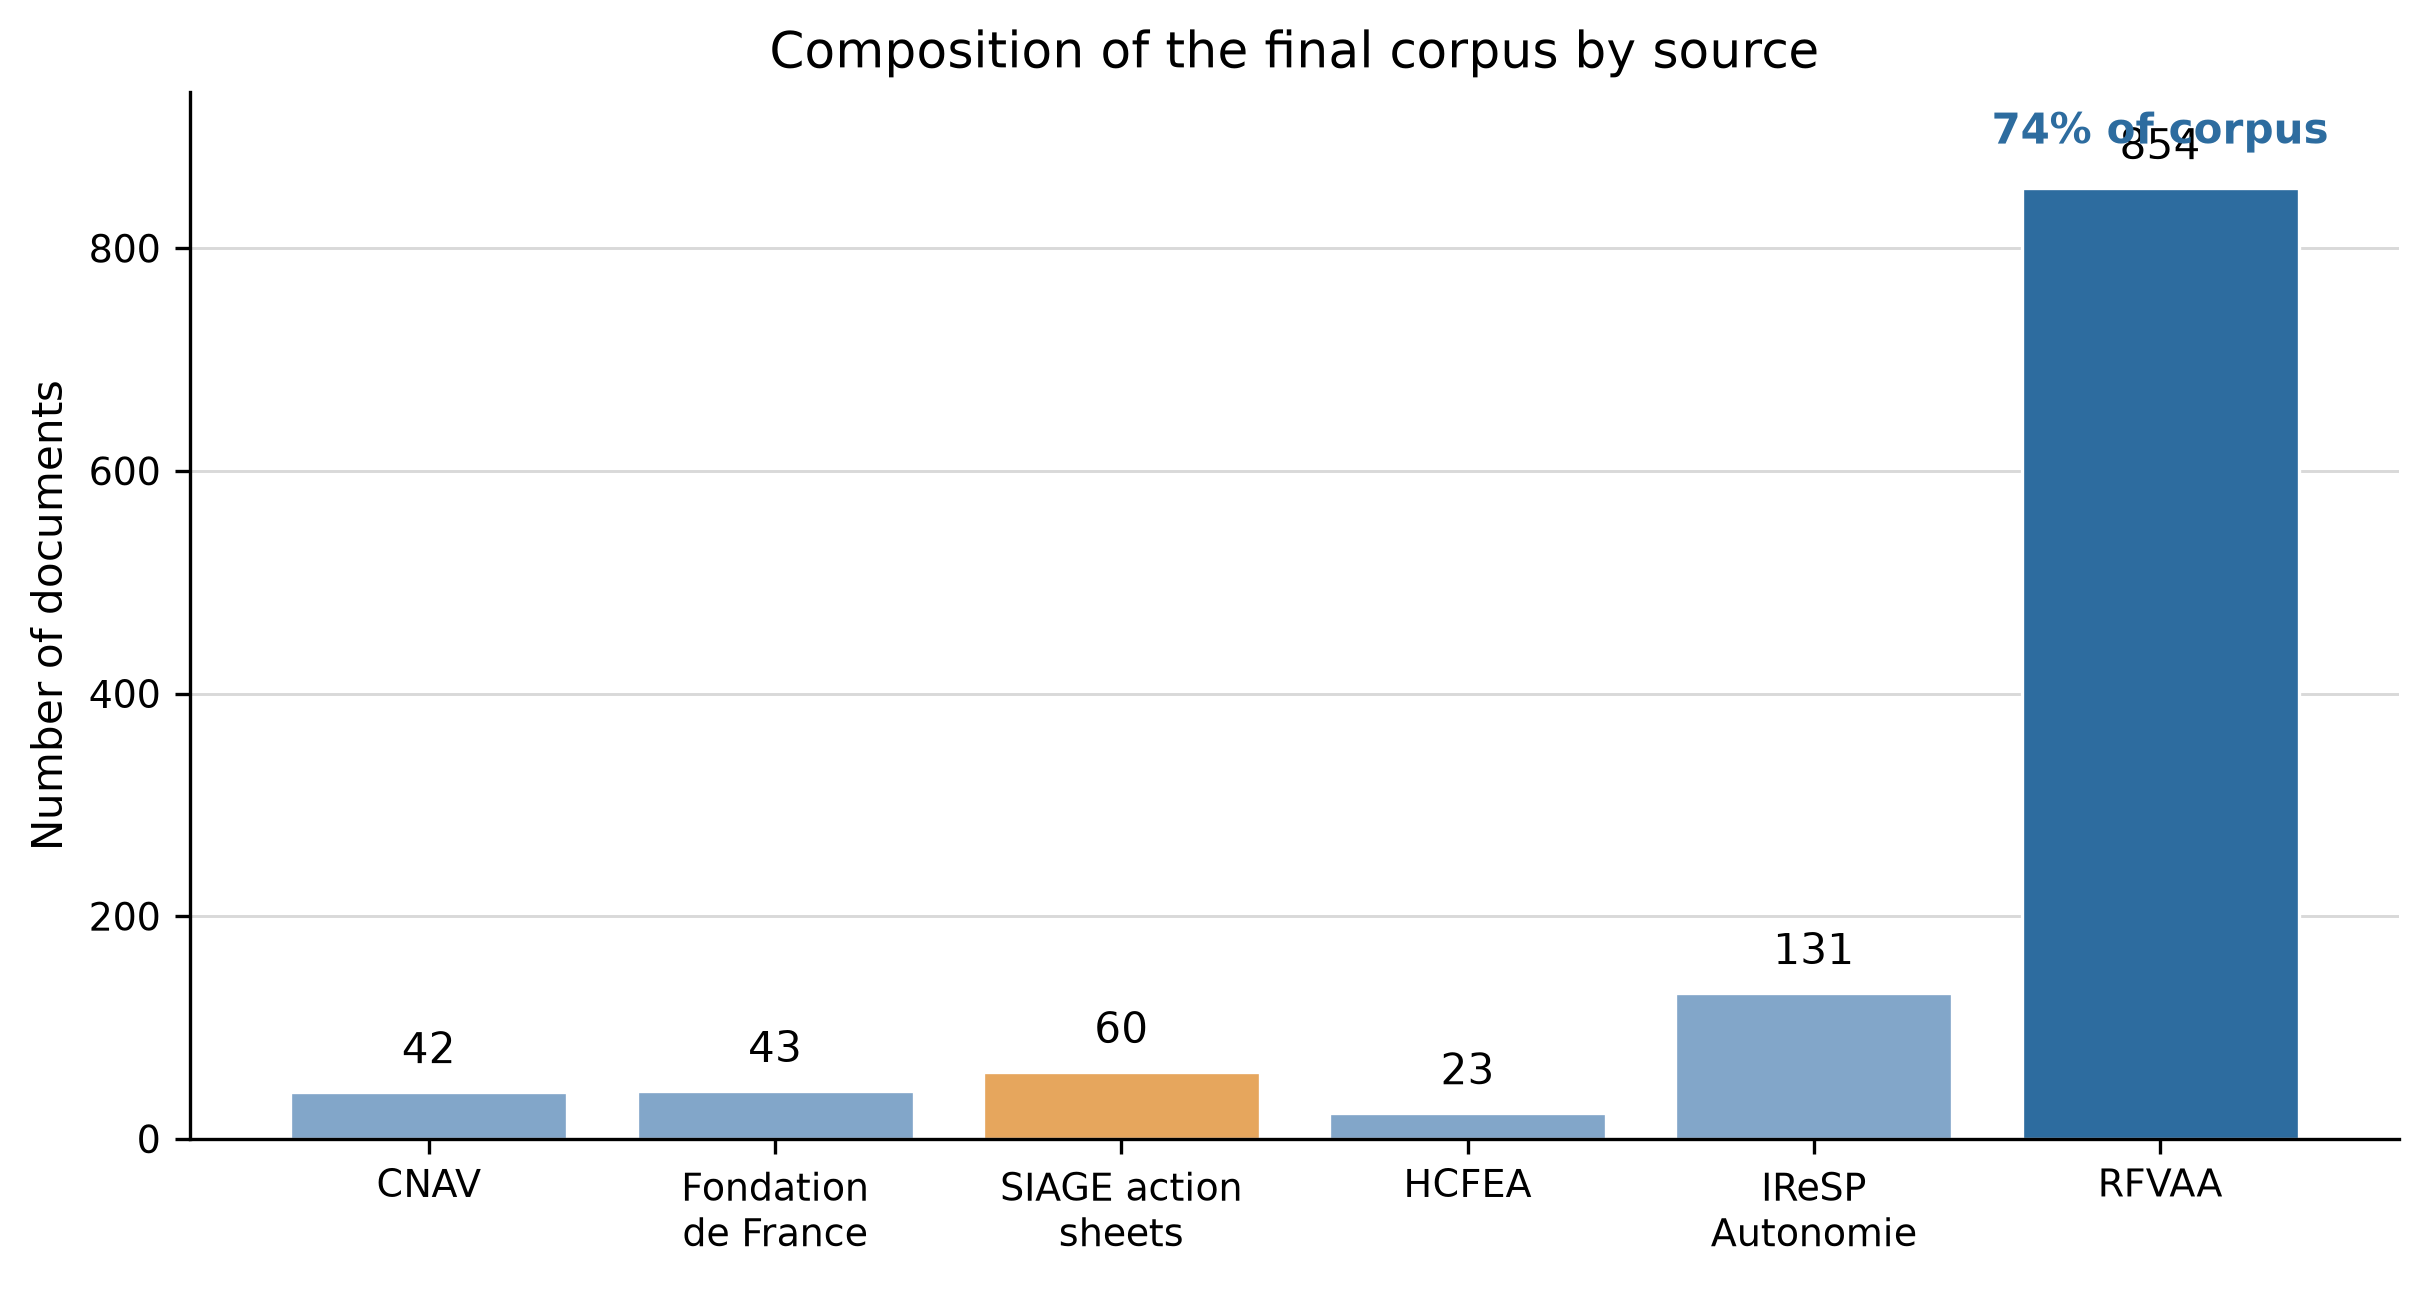
\includegraphics[width=0.82\textwidth]{Figures/corpus-source-composition.png}
    \caption{Composition of the final corpus by source. RFVAA represents 854
    of the 1,153 documents (approximately 74\%), so source composition must be
    considered when interpreting descriptive distributions.}
    \label{fig:corpus-source-composition}
\end{figure}

% Insert the second figure in the Evaluation chapter, immediately after
% Table~\ref{tab:llm-judgment-results}. It may precede the source-level table.

\begin{figure}[H]
    \centering
    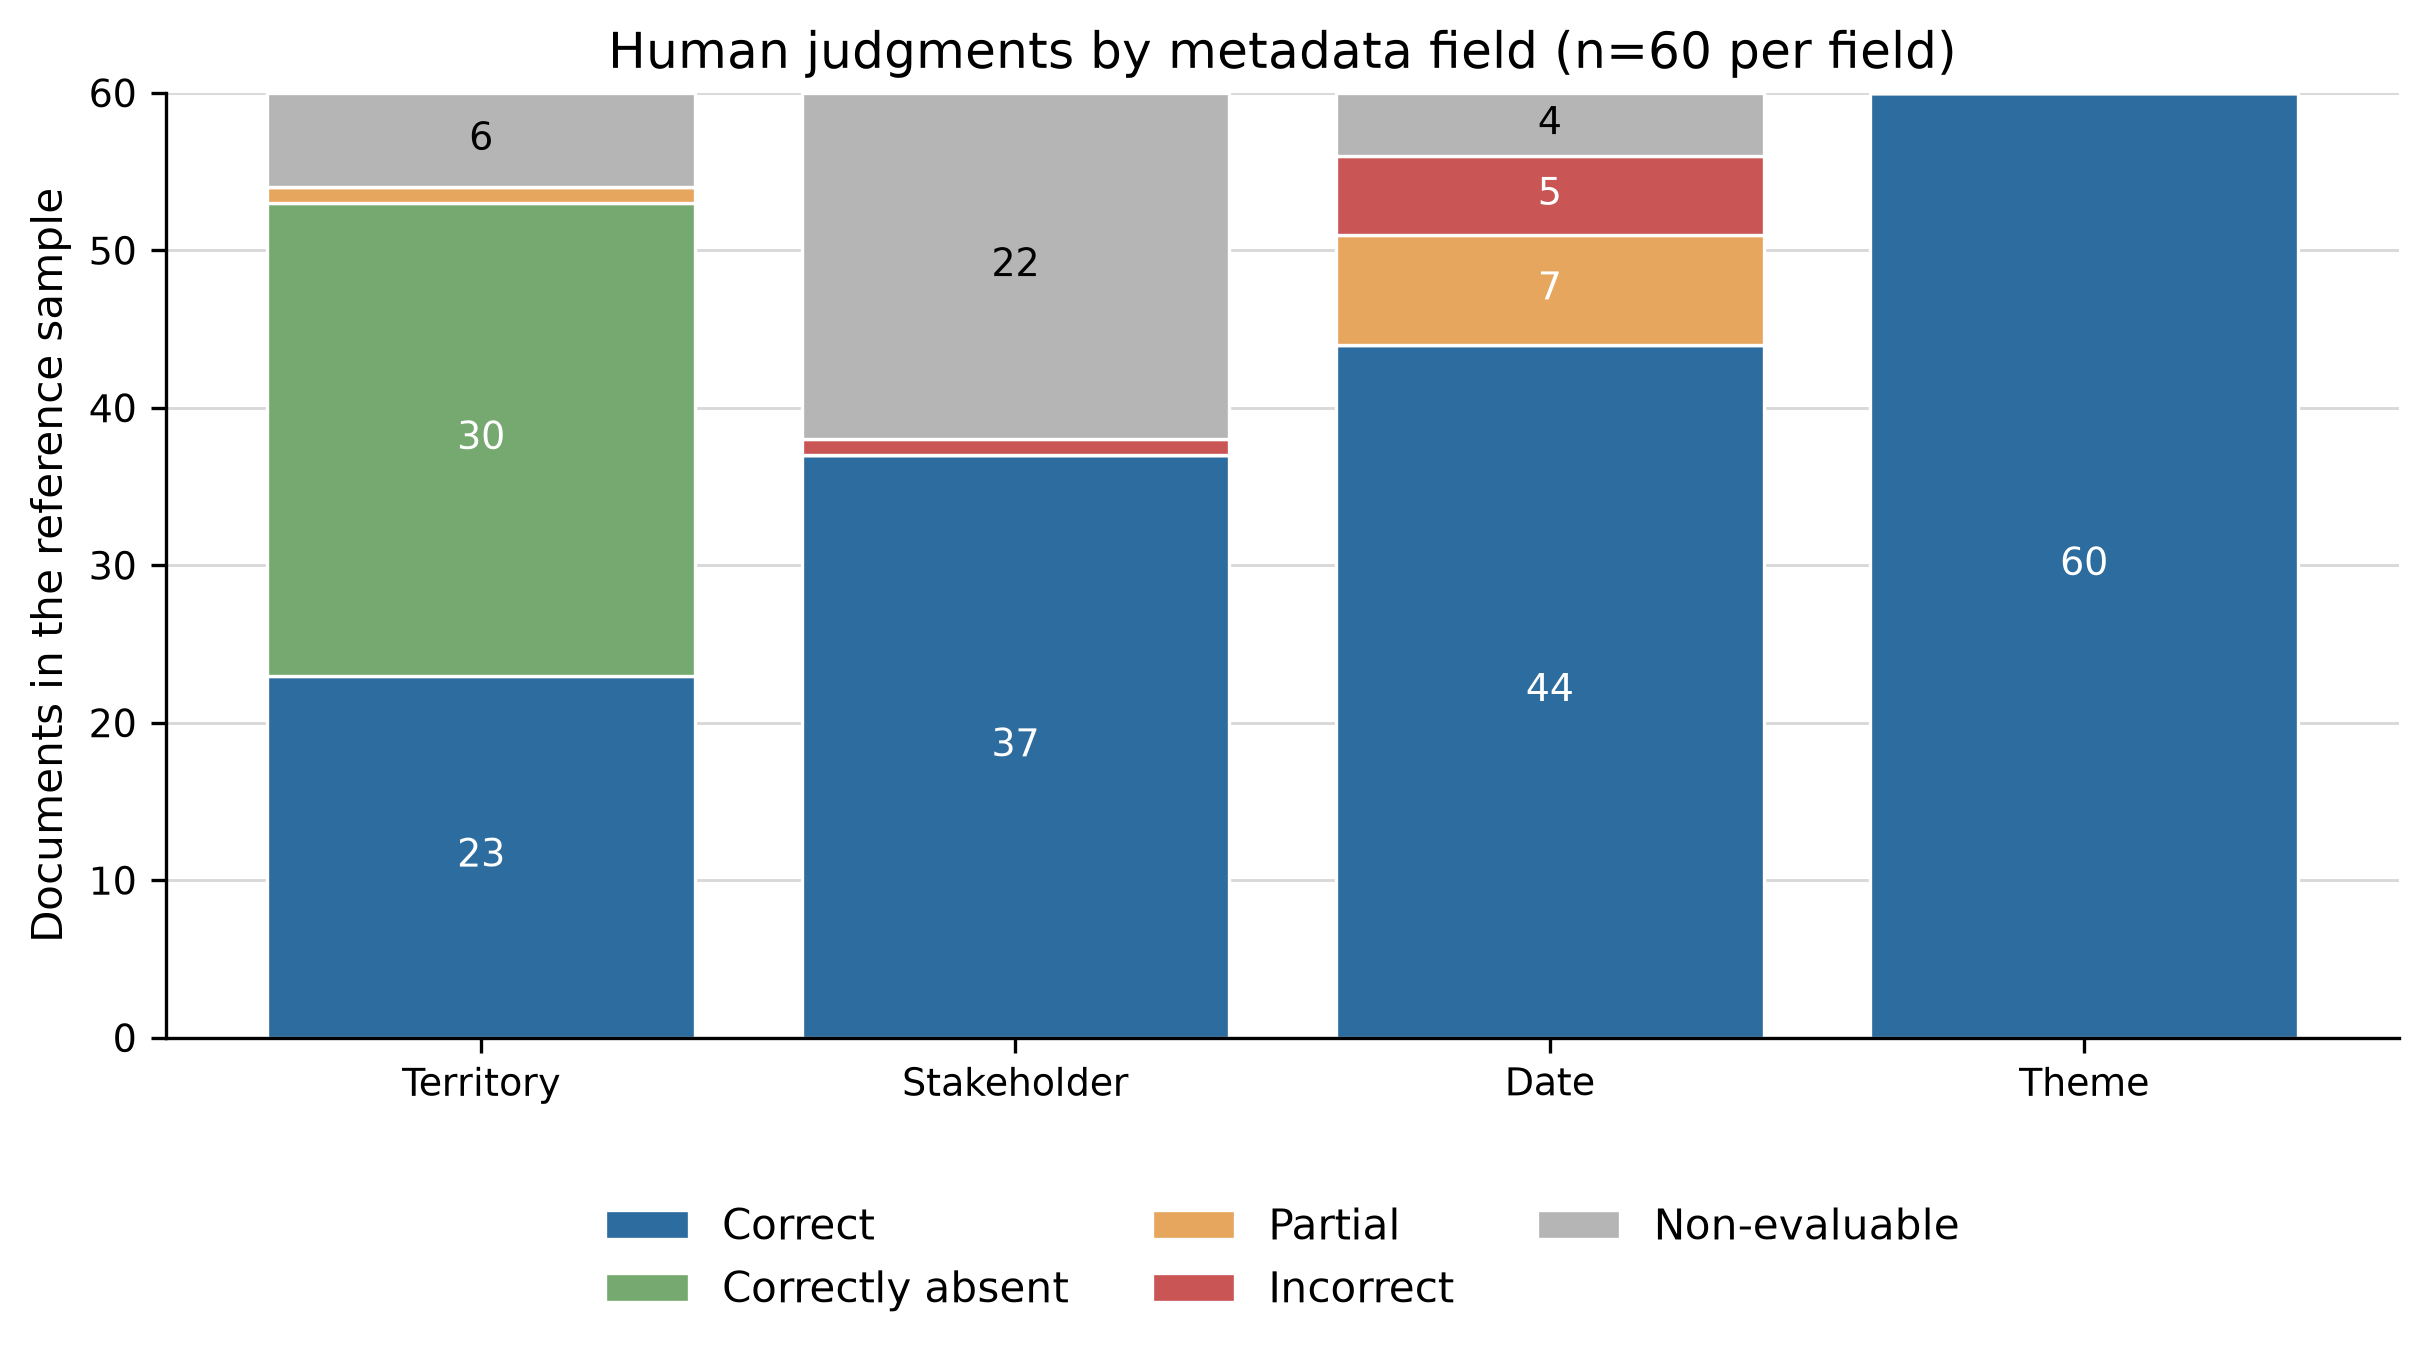
\includegraphics[width=0.82\textwidth]{Figures/human-judgment-distribution.png}
    \caption{Distribution of human judgments for four extracted metadata
    fields. Correctly absent predictions are treated as accepted because the
    source did not provide sufficient information to fill the corresponding
    field.}
    \label{fig:human-judgment-distribution}
\end{figure}
